\chapter{Posterior of Bayesian Hierachical model}
\label{ap:bayesian}
Here we show how to obtain the posterior covariance and mean of our hierarchical Bayesian model in \ref{eq:prior} - \ref{eq:post}.
We do not consider the hyper-parameters and start with the joint probaility distribution of $(\bm{x}^T,\bm{y}^T)^T$, where $\bm{x} \in \mathcal{X}$ and $\bm{y} \in \mathcal{Y}$ do not intersect.
For more details we refer to Chapter 2 in \cite{bishop2006pattern} and to the book of Rue and Held \cite{rue2005gaussian}.

The exponent of the normal Gaussian can be rewritten into:
\begin{align}
\label{eq:gauss}
    -\frac{1}{2}(\bm{x} - \bm{\mu})^T \bm{Q} (\bm{x} - \bm{\mu}) = - \frac{1}{2} \bm{x}^T \bm{Q} \bm{x} + \bm{x}^T \bm{Q} \bm{\mu} + \text{const.}
\end{align}
We like to bring the joint distribution into a similar form so that we can compare the linear and second order terms and find the precision matrix and mean of the joint distribution.


In general the joint distribution to find the experssino for the postiror dostrbution

We can express this posterior through the likelihood and prior probability by Bayesian theorem, with a constant and positive normalization constant:
\begin{equation}
    \pi(\bm{x} |\bm{y}) \propto \pi( \bm{y} | \bm{x} )  \pi(\bm{x} )
\end{equation}
Taking the logarithmic function of this formulation we can find an expression for the the posterior covariance, with the $\text{Var}(\bm{x}) = \bm{Q_x}^{-1}$ and $\text{Var}(\bm{y}) = \bm{Q_y}^{-1}$.
\begin{align}
\ln{\pi(\bm{x|y})} \propto&  \ln{ \pi( \bm{y} | \bm{x} ) } + \ln{\pi( \bm{x} ) }\\
=& - \frac{1}{2} (\bm{x} - \bm{\mu} )^T \bm{Q_x} (\bm{x} - \bm{\mu} ) - \frac{1}{2} (\bm{y} - \bm{Ax} )^T \bm{Q_y} (\bm{y} - \bm{Ax} )    \\
=& - \frac{1}{2} \bigg[ \bm{x}^T \big[ \bm{Q_x} + \bm{A}^T \bm{Q_y} \bm{A} \big] \bm{x}  + \bm{x}^T \big[ - \bm{A}^T \bm{Q_y} \big] \bm{y} \\
&+ \bm{y}^T \big[ - \bm{Q_y A} \big] \bm{x} + \bm{y}^T \big[ \bm{Q_y} \big] \bm{y} - 2 \bm{x}^T \bm{Q_x \mu }  \bigg] + \text{const.}
\end{align}

Hence we deal with a Gaussian distribution, we consider second order terms only and rearrange to the precision matrix.
\begin{align}
    &- \frac{1}{2} \begin{bmatrix}
        \bm{x}^T \big[ \bm{Q_x} + \bm{F}^T \bm{Q_y} \bm{F} \big]  + \bm{y}^T \big[ - \bm{Q_y F} \big] & \bm{y}^T \big[ \bm{Q_y} \big] + \bm{x}^T \big[ - \bm{F}^T \bm{Q_y} \big] 
    \end{bmatrix}  \begin{bmatrix}
        \bm{x} \\ \bm{y}
    \end{bmatrix} \\
    =& \begin{bmatrix}
        \bm{x}^T & \bm{y}^T
    \end{bmatrix} 
    \underbrace{\begin{bmatrix}
        \bm{Q}_x + \bm{F}^T \bm{Q}_y \bm{F} & - \bm{F}^T \bm{Q}_y \\
        -\bm{Q}_y \bm{F} & \bm{Q}_y
    \end{bmatrix}}_\text{precision matrix} \begin{bmatrix}
        \bm{x} \\ \bm{y}
    \end{bmatrix} 
\end{align}
We denote the precision matrix of the joint field as:
\begin{align}
    \bm{Q}_{xy} = \begin{bmatrix}
        \bm{Q}_{aa} & \bm{Q}_{ab} \\
        \bm{Q}_{ba} & \bm{Q}_{bb}
    \end{bmatrix} = 
    \begin{bmatrix}
        \bm{Q}_x + \bm{F}^T \bm{Q}_y \bm{F} & - \bm{F}^T \bm{Q}_y \\
        -\bm{Q}_y \bm{F} & \bm{Q}_y
    \end{bmatrix}
\end{align}

The mean is defined through the linear term.
\begin{align}
    \frac{- 2 \bm{x}^T \bm{Q_x \mu } }{-2} = \begin{bmatrix}
        \bm{x}^T & 0
    \end{bmatrix} \begin{bmatrix}
        \bm{Q_x \mu}\\ 0
    \end{bmatrix} 
    \end{align} 
Comparing to the linear term of Equation \ref{eq:gauss} we can formulate an expression for the joint mean:
    \begin{align}
    \Rightarrow \bm{\mu_{xy}} = \bm{Q}_{\bm{x}\bm{y}}^{-1}   \begin{bmatrix}
        \bm{Q_x \mu}\\ 0
    \end{bmatrix}
\end{align}
The mean of the conditional distribution $\bm{x}|\bm{y}$ is given by:
\begin{align}
\bm{\mu}_{\bm{x}|\bm{y}} &= \bm{\mu}_{\bm{x}} + \bm{Q}^{-1}_{ba} \bm{Q}_{ab} (\bm{x} - \bm{\mu}_{\bm{y}}) \\
\bm{\mu}_{\bm{x}|\bm{y}} &= \bm{\mu} +  ( \bm{Q}_x + \bm{F}^T \bm{Q}_y \bm{F} )^{-1} \bm{F}^T \bm{Q}_y ( \bm{x} - \bm{F \mu} ) \, ,
\end{align}
and the covariance of $\bm{x}|\bm{y}$ is given by:
\begin{align}
   \bm{Q}_{\bm{x}|\bm{y}} =  \bm{Q}_{aa} = \bm{Q}_x + \bm{F}^T \bm{Q}_y \bm{F} \, ,
\end{align}
as illustrated through Theorem 2.5 in \cite{rue2005gaussian}.


\chapter{Convergence of the Metropolis-Hastings}
\label{ap:MetroHast}

If we show that the detailed balance condition holds and that the state space is irreducible and aperiodic under the transition matrix $\bm{P}$, we generate a Markov chain with a unique stationary distribution proportional to $\pi (\bm{x} , \bm{\theta} | \bm{y})$.
Since the posterior is strictly positive $\pi (\bm{x} , \bm{\theta} | \bm{y}) \geq 0$ on the finite state space $\Omega(\mathcal{X},\mathcal{\theta})$ the generated chain is irreducable.
Further, it is possible to reject any proposed state and stay in the current state, which leads to aperiodicity.
The detailed balance holds for the case that $\bm{j} = \bm{i}$, but if $\bm{j} \neq \bm{i}$ it is not trivial.
In case we accept $\{ \bm{x}, \bm{\theta} \}^{(n+1)} = \bm{j}$ as the new state we have $ \pi(\bm{j} | \bm{y})  g(\bm{i}|\bm{j})> \pi(\bm{i} | \bm{y})  g(\bm{j}|\bm{i})$.
This gives us $\alpha(\bm{j}|\bm{i}) = 1$ and $\alpha(\bm{i}|\bm{j}) = \frac{\pi_{\bm{i}} g(\bm{j}|\bm{i})}{\pi_{\bm{j}} g(\bm{i}|\bm{j})}$ and satisfies the detailed balance:
\begin{align*}
    \cancel{\pi_{\bm{j}}}  \frac{\pi_{\bm{i}}}{\cancel{\pi_{\bm{j}}}} g(\bm{j}|\bm{i}) &= \pi_{\bm{i}} g(\bm{j}|\bm{i}) \quad .
\end{align*}
If $ \pi(\bm{j} | \bm{y})  g(\bm{i}|\bm{j}) < \pi(\bm{i} | \bm{y})  g(\bm{j}|\bm{i})$ then $\alpha(\bm{i}|\bm{j}) = 1$
and $\alpha(\bm{j}|\bm{i}) = \frac{\pi_{\bm{j}} g(\bm{i}|\bm{j})}{\pi_{\bm{i}} g(\bm{j}|\bm{i})}$, this satisfies the detailed balance as well.

In conclusion the Metropolis-Hastings algorithm samples from a unique distribution proportional to the posterior distribution. 

\chapter{Randomize then Optimize - RTO}
\label{ap:RTO}

\begin{align}
    \pi(\bm{x}|\bm{y}, \bm{\theta} ) &\propto \pi(\bm{y} | \bm{x} , \bm{\theta} ) \pi(\bm{x}| \bm{\theta}) \\
   &\propto \exp \Big[  ( \bm{F x} - \bm{y})^T \bm{\Sigma}^{-1}( \bm{F x} - \bm{y}) + (\bm{x} -\bm{\mu} )^T \bm{Q} (\bm{x} -\bm{\mu})\Big] \\
   &= \exp  \lVert \hat{\bm{F}} \bm{x} - \hat{\bm{y}} \rVert^2 
\end{align}
where 
\begin{align}
\hat{\bm{F}} = 
    \begin{bmatrix}
         \bm{\Sigma}^{-1/2} \bm{F}\\
    \bm{Q}^{1/2}
    \end{bmatrix} \, , \quad \hat{\bm{y}} = 
    \begin{bmatrix}
        \bm{\Sigma}^{-1/2} \bm{y} \\
        \bm{Q}^{1/2}\bm{\mu}
    \end{bmatrix}
\end{align}

One sample from the posterior can be computed by minimizing the following with respect to $\bm{x}$
\begin{align}
    \bm{x} = \arg \min_{\hat{\bm{x}}} \lVert \hat{\bm{F}} \hat{\bm{x}} - ( \hat{\bm{y}} + \bm{\eta} ) \rVert^2 , \quad \bm{\eta} \sim \mathcal{N}(\bm{0}, \mathbf{I})
\end{align}

We can solve this and rewrite to
\begin{align}
    \frac{\partial}{\partial \bm{x} }  \big[   (\hat{\bm{F}} \bm{x} - ( \hat{\bm{y}} + \bm{\eta} )^T (\hat{\bm{F}} \bm{x} - ( \hat{\bm{y}} + \bm{\eta} ) \big] &= 0 \\
    \Leftrightarrow \bm{x}^T \hat{\bm{F}}^T  \hat{\bm{F}} + \hat{\bm{F}}^T \hat{\bm{F}} \bm{x} -  \hat{\bm{F}}^T ( \hat{\bm{y}} + \bm{\eta} )- ( \hat{\bm{y}} + \bm{\eta} )^T  \hat{\bm{F}} \bm{x}  &= 0
\end{align}
We can argue through the symmetry of the inner product that and the symmetry of the precision matrix
\begin{align}
    \hat{\bm{F}}^T \hat{\bm{F}} \bm{x} &= \hat{\bm{F}}^T ( \hat{\bm{y}} - \bm{\eta}) \\
    \Leftrightarrow  (\bm{F}^T \bm{Q_y} \bm{F}+
    \bm{Q} ) \bm{x} &= \bm{F}^T \bm{Q_y} \bm{y} +  \bm{Q} \bm{\mu} - \hat{\bm{F}}^T  \bm{\eta}  
\end{align}
If we substitute $ - \hat{\bm{F}}^T  \bm{\eta}  = \bm{v}_1 + \bm{v}_2$ we end up with 
\begin{align}
    (\bm{F}^T \bm{\Sigma}^{-1} \bm{F}+
    \bm{Q} ) \bm{x} &= \bm{F}^T \bm{\Sigma}^{-1} \bm{y} +  \bm{Q} \bm{\mu} + \bm{v}_1 + \bm{v}_2
\end{align}
where $\bm{v}_1 \sim \mathcal{N}(\bm{0}, \bm{F}^T \bm{\Sigma}^{-1} \bm{F}) $ and $\bm{v}_2 \sim \mathcal{N}(\bm{0}, \bm{Q} )$ are independent random variables.
mayeb introduce... $x^2$ time nomral variubale


\chapter{Inverting Matrices - QR factorization}


\chapter{Taylor expansion of  $g(\lambda)$}
\label{ap:taylor}
We Taylor expand the function $g(\lambda)$ around $\lambda = \lambda'  - \Delta \lambda$
\begin{align}
    g(\lambda) = \ln \det \underbrace{(\bm{F}^T  \bm{F} + \lambda \bm{L})}_{\bm{B}}
\end{align}
\begin{align}
       g(\lambda') -    g(\lambda) &=  \ln \det ( \bm{F}^T  \bm{F} + \lambda' \bm{L}) -  \ln \det (\bm{F}^T  \bm{F} + \lambda \bm{L}) \\
    &=  \ln \det \Bigg[ \frac{(\bm{F}^T  \bm{F} + (\lambda + \Delta \lambda) \bm{L}) }{ ( \bm{F}^T  \bm{F} + \lambda \bm{L}) } \Bigg]  \\
       &=  \ln \det \Bigg[ 1 + \frac{ \Delta \lambda \bm{L} }{ \bm{B} } \Bigg]\\
       & = \sum_{r = 1}^{\infty} \frac{(-1)^{r+1}}{r !}\text{tr} (   (\bm{B}^{-1}  \bm{L} )^r  )  (\Delta \lambda)^r
\end{align}, where we use the identity from \cite{gohberg2012traces} at page 29.
So the derivatives of $g(\lambda)$ are:
\begin{align}
    g^{(r)} ( \lambda) =&  (-1)^{r+1} \, \text{tr} \big( (\bm{B}^{-1}\bm{ L })^r \big)\\
\approx& (-1)^{r+1} \sum^p_{k=1} \bm{z_k}^T (\bm{B}^{-1} \bm{L} )^r \bm{z_k}  
\end{align} 
Here we use a Monte Carlo estimate and draw $p$ vectors $\bm{z_k} \in \mathbb{R}^n $, where each vector element $z_i \overset{\text{i.i.d.}}{\sim} \mathcal{U} ( \{ -1, 1 \} )$ and $i = 1 , \dots, n$.

\chapter{Radiation transfer and absorption line shape}
\label{ap:RTE}


\chapter{whispering gallery resonator}
\label{ap:resonator}


\begin{figure}
\centering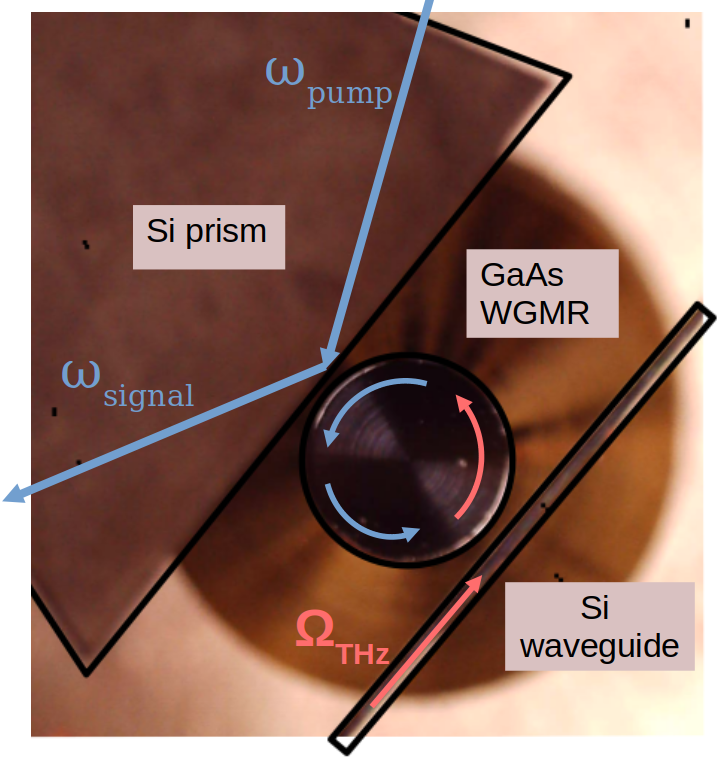
\includegraphics[width=0.7\textwidth]{GaAs_setup4.png} 
\caption[whispering gallery resonator]{whispering gallery resonator}
\label{fig:GaAsRes}
\end{figure}